\documentclass[12pt,a4paper,oneside]{article}

\usepackage[utf8]{inputenc}
\usepackage[portuguese]{babel}
\usepackage[T1]{fontenc}
\usepackage{amsmath}
\usepackage{amsfonts}
\usepackage{amssymb}
\usepackage{graphicx}

\usepackage{xcolor}
% Definindo novas cores
\definecolor{verde}{rgb}{0.25,0.5,0.35}
\definecolor{jpurple}{rgb}{0.5,0,0.35}
% Configurando layout para mostrar codigos Java
\usepackage{listings}
\lstset{
  language=Java,
  basicstyle=\ttfamily\small, 
  keywordstyle=\color{jpurple}\bfseries,
  stringstyle=\color{red},
  commentstyle=\color{verde},
  morecomment=[s][\color{blue}]{/**}{*/},
  extendedchars=true, 
  showspaces=false, 
  showstringspaces=false, 
  numbers=left,
  numberstyle=\tiny,
  breaklines=true, 
  backgroundcolor=\color{cyan!10}, 
  breakautoindent=true, 
  captionpos=b,
  xleftmargin=0pt,
  tabsize=4,
  escapeinside=||
}

\author{\\Universidade Federal de Goiás (UFG) - Regional Jataí\\Bacharelado em Ciência da Computação \\Teoria dos Grafos \\Esdras Lins Bispo Jr.}

\title{\sc \huge Quarto Teste}

\date{08 de agosto de 2016}

\begin{document}

\maketitle

{\bf ORIENTAÇÕES PARA A RESOLUÇÃO}

\footnotesize

\begin{itemize}
	\item A avaliação é individual, sem consulta;
	\item A pontuação máxima desta avaliação é 10,0 (dez) pontos, sendo uma das 05 (cinco) componentes que formarão a média final da disciplina: dois testes, duas provas e exercícios;
	\item A média final ($MF$) será calculada assim como se segue
	\begin{eqnarray}
		MF & = & MIN(10, S) \nonumber \\
		S & = & (\sum_{i=1}^{4} 0,2.T_i ) + 0,2.P  + EB \nonumber
	\end{eqnarray}
	em que 
	\begin{itemize}
		\item $S$ é o somatório da pontuação de todas as avaliações,
		\item $T_i$ é a pontuação obtida no teste $i$,
		\item $P$ é a pontuação obtida na prova, e
		\item $EB$ é a pontuação total dos exercícios-bônus.
	\end{itemize}
	\item O conteúdo exigido compreende os seguintes pontos apresentados no Plano de Ensino da disciplina: (7) Isomorfismo, (8) Coloração e (10) Outros tópicos.
\end{itemize}

\begin{center}
	\fbox{\large Nome: \hspace{10cm}}
	\fbox{\large Assinatura: \hspace{9cm}}
\end{center}

\newpage

\normalsize

\begin{enumerate}

	\item (5,0 pt) [E 2.18] O seguinte algoritmo se propõe a decidir se dois grafos, $G$ e $H$, são isomorfos:
		\begin{itemize}
			\item[] se $n(G) \not= n(H)$ então $G$ e $H$ não são isomorfos;
				\begin{itemize}
					\item[] se $m(G) \not= m(H$) então $G$ e $H$ não são isomorfos;
					\begin{itemize}
						\item[]  se $|{v \in V_G : d_G (v) = i}|$ $\not=$ $|{v \in V_H : d_H (v) = i}|$ \\
						para algum $i$, então G e H não são isomorfos;
					\end{itemize}
				\end{itemize}
			\item[] em todos os demais casos, G é isomorfo a H.
		\end{itemize}
		
	Discuta o algoritmo, justificando se o mesmo decide ou não corretamente o isomorfismo entre grafos.
	
	\item (5,0 pt) [(DG) E 1.9] (Adaptação) A função {\tt DIGRAPHreverse()} reverte (inverte?) um digrafo $G$, ou seja, constroi um digrafo cujos arcos têm direção contrária aos de $G$ (veja na figura abaixo). Entretanto, há três trechos no código que estão faltando. Escreva o código deste três trechos.
	\begin{center}
		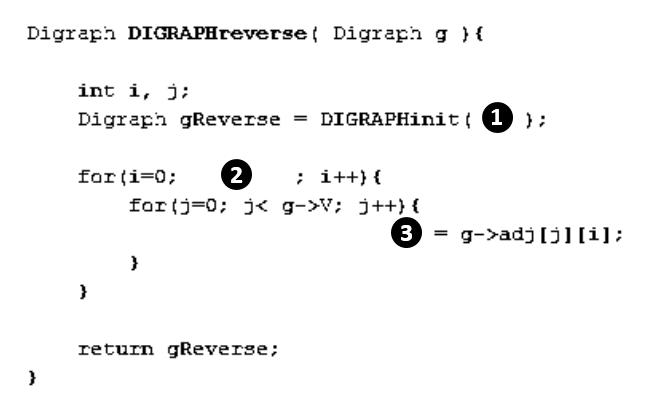
\includegraphics[width=0.8\textwidth]{images/reverse2.png}
	\end{center}
	
	\end{enumerate}
\end{document}